\chapter{Implementation}
	
\subsection{DCE-MRI data acquisition}
The data used in this project were acquired on 32 channel 1.5 T whole-body scanner (Siemens Magnetom Avanto \cite{simens}).
The  images covering kidneys and aorta were continuously acquired every 2.3 s for approximately 6 min in coronal-oblique plane.
Each of 74 time volumes consisted of 30 slices.
The aquisition matrix was 192x192 whereas the voxel size was equal to 2.2x2.2x3 mm$^3$
More information about aquisition of DCE-MRI data used in this project can be found in \cite{eikefjord2017dynamic}.

\subsection{Motion correction}
One of the first fundamental problem encountered during DCE-MRI analysis is misalignment of 3D volumes across time slices. This misalignment of organs is a result of the patiens's respiratory motion as well as the heartbeat and bowel peristalsis and is unavoidable during examination. Studies have shown that even slight misalignment can lead to significant differences in intensity time-courses \cite{KidneySubsegmentation} and thus, motion correction of time series is essential for further analysis.

In order to remove motion artifact, all files were motion-corrected across time points. For this purpose R programming language for statistical computing and graphics was used \cite{R} together with the package ANTsR \cite{ANTsR}, which provides quantification tools for biomedical images. As an initial step, for every time series, the algorithm extracted 3D volumes. Each extracted volume corresponded to data obtained in one time point. Next, the average image of the temporal volumes was calculated, which was treated as a mask for image registration. Every temporal volume was then aligned to the mask and at the end they were combined back together into 4D time series. 
 
\subsection{Manual labelling of kidneys and aorta} 
\label{subsec:labelling}
In the next step, labels of both left and right kidney were created. For this purpose, 3D volumes were extracted for every time frame and the image with maximal signal enhancement was chosen (usually between 12--17 time slice). On this image, left and right kidney were manually delineated in coronal plane using ITK-Snap software \cite{itk-snap}. Additionally, few voxels of aorta (15--20) were labelled. So obtained labels were then propagated across the time points. All further analysis was implemented in Python programming language v. 3.6 \cite{python}.  
 
\subsection{Pelvis segmentation}
\label{subsec:pelvis}
Due to the fact that glomelular filtration takes place in renal renal parenchyma, pelvis had to be removed from further analysis. 

Resulting from the physiology of the process, the three renal compartments (cortex, medulla, pelvis) can be distinguished from each other on the basis of their time courses, as shown on Figure~\ref{fig:timecourses}. Depending on the compartment, the rapid enhancement of the signal occurs in different period, which makes the shapes of the time intensity curves very unique.
From the \ref{fig:timecourses} it can be seen that the biggest variation is observed between pelvis and two other renal compartments.    Consequently, it can be separated by unsupervised clustering. 

\begin{figure}[H]
	\centering
	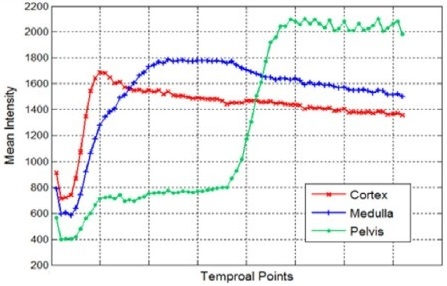
\includegraphics[width = \columnwidth]{img/timecourses}
	\caption{Kidney compartments timecourses  \cite{KidneySubsegmentation}.}
	\label{fig:timecourses}
\end{figure}
 
\subsubsection{Dimensionality reduction}
Raw DCE-MRI data usually has high dimension, which results in computational complexity, and thus memory and time consumption as well as numerical problems. What is more it contains a lot of noises \cite{KidneySubsegmentation}. To overcome this problems, the Principal Component Analysis (PCA) \cite{wold1987principal} was applied.

PCA is a statistical procedure, which transforms the number of related features into smaller set of uncorrelated variables  \cite{pca}. These so called principal components (PCs) are a linear combination of the original variables \cite{dunteman1989principal}. As a result, after rotating the feature space, the first PC contains most variance and so on. In this way the dominant patterns are extracted while the noises are reduced \cite{wold1987principal}.

Applying the theory to practice, each voxel belonging to the kidneys, initially described by 74 features (value of the signal intensity in 74 time points) was described by 10 PCs.

\subsubsection{Clustering}
In the next step, the k-means clustering \cite{kmeans} was performed in order to separate voxels into two groups: pelvis and renal parenchyma.  

The k-means is an unsupervised clustering algorithm aiming to minimize the square error function given by:

\begin{equation}
	\label{eq:kmeans}
	J = \sum_{j=1}^{k}\sum_{i=1}^{n}(||x_i-c_j||)^2,
\end{equation}
where $||x_i-c_j||$ is  the Euclidean distance between a data point $x_i$ and the cluster centre $c_j$ of k predefined clusters.

For each of two clusters, in which signal intensity reaches its maximum $T_{max}$ was calculated. 
Following the assumption that $T_{max\_pelvis}>T_{max\_parenchyma}$, the cluster with greater $T_{max}$ was marked as the pelvis and removed from the region of interest (ROI).

\subsection{Kidneys segmentation using deep learning}

As mentioned before, the main goal of the overall project is to develop method not requiring the interference of the human at any stage and thus being fully objective, which is contrary with previously described steps. In target method, the steps descried in sections \ref{subsec:labelling} - \ref{subsec:pelvis} will be replaced by deep learning techniques. The designed neural networks should not require registration of the images, which is usually the most inconvenient step. Not only is it very time-consuming (motion correction of the one time series used in the project lasts \textasciitilde 6h) but also it causes loss of information. As a~result, the method will enable fast and efficient automated GFR estimation directly from the DCE-MRI without any previous preprocessing.
Although applying deep learning is still under intensive development, current studies already have showed promising results. What was achieved so far, is segmentation of the both left and right kidney from raw DCE-MRI images using convolutional neural network. 

Convolutional Neural Networks (CNN) were inspired by the architecture of the animal visual cortex and are specifically suitable for image recognition. It was shown that numerous neurons in the visual cortex are sensitive only to the stimuli located in the small limited region of the visual field. In short terms, these neurons have small local receptive fields, which can overlap and all together cover whole visual field. What is more, certain neurons are activated only by horizontal lines, whereas the others reacts to these of different orientations.
Furtermore, some neurons with bigger receptive fields responds to the more complex patterns being the assembly of the lower-level patterns, which leads to the conclusion that the higher-level neurons are based on the outputs of neighbouring lower-level neurons \cite{hubel1968receptive,handson}.  The described complex system composed of the neurons ordered in a columnar fashion is able to detect all kinds of patterns in whole visual field creating the visual perception. The above idea is shown on Figure \ref{fig:visual_cortex}. 
 

\begin{figure*}
	\centering
	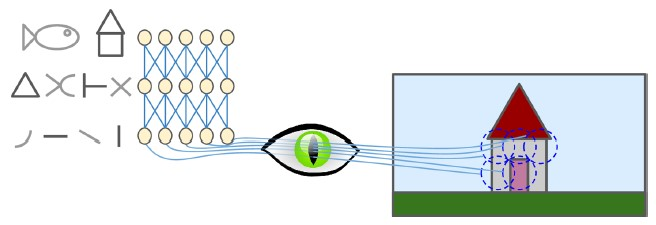
\includegraphics[width = \linewidth]{img/visual_cortex}
	\caption{Local receptive fields in the visual cortex \cite{handson}.}
	\label{fig:visual_cortex}
\end{figure*}

From the finding of the studies on visual cortex convolutional neural networks emerged. Unlike the traditional neural networks, their architecture incorporates multiple convolutional layers, neurons of which  connect to the subregions of the previous layers instead of being fully-connected. The neurons are not sensitive to the areas outside of these subregions in the image.
Each of the layer learn to recognise different feature. The deeper the layer is, the more detailed 

The network has a dual pathway architecture incorporating both local and global information in the volumes. It consist of \color{red}(?) \color{black} layers.
The idea of transfer learning was applied. 

\begin{figure*}
	\centering
	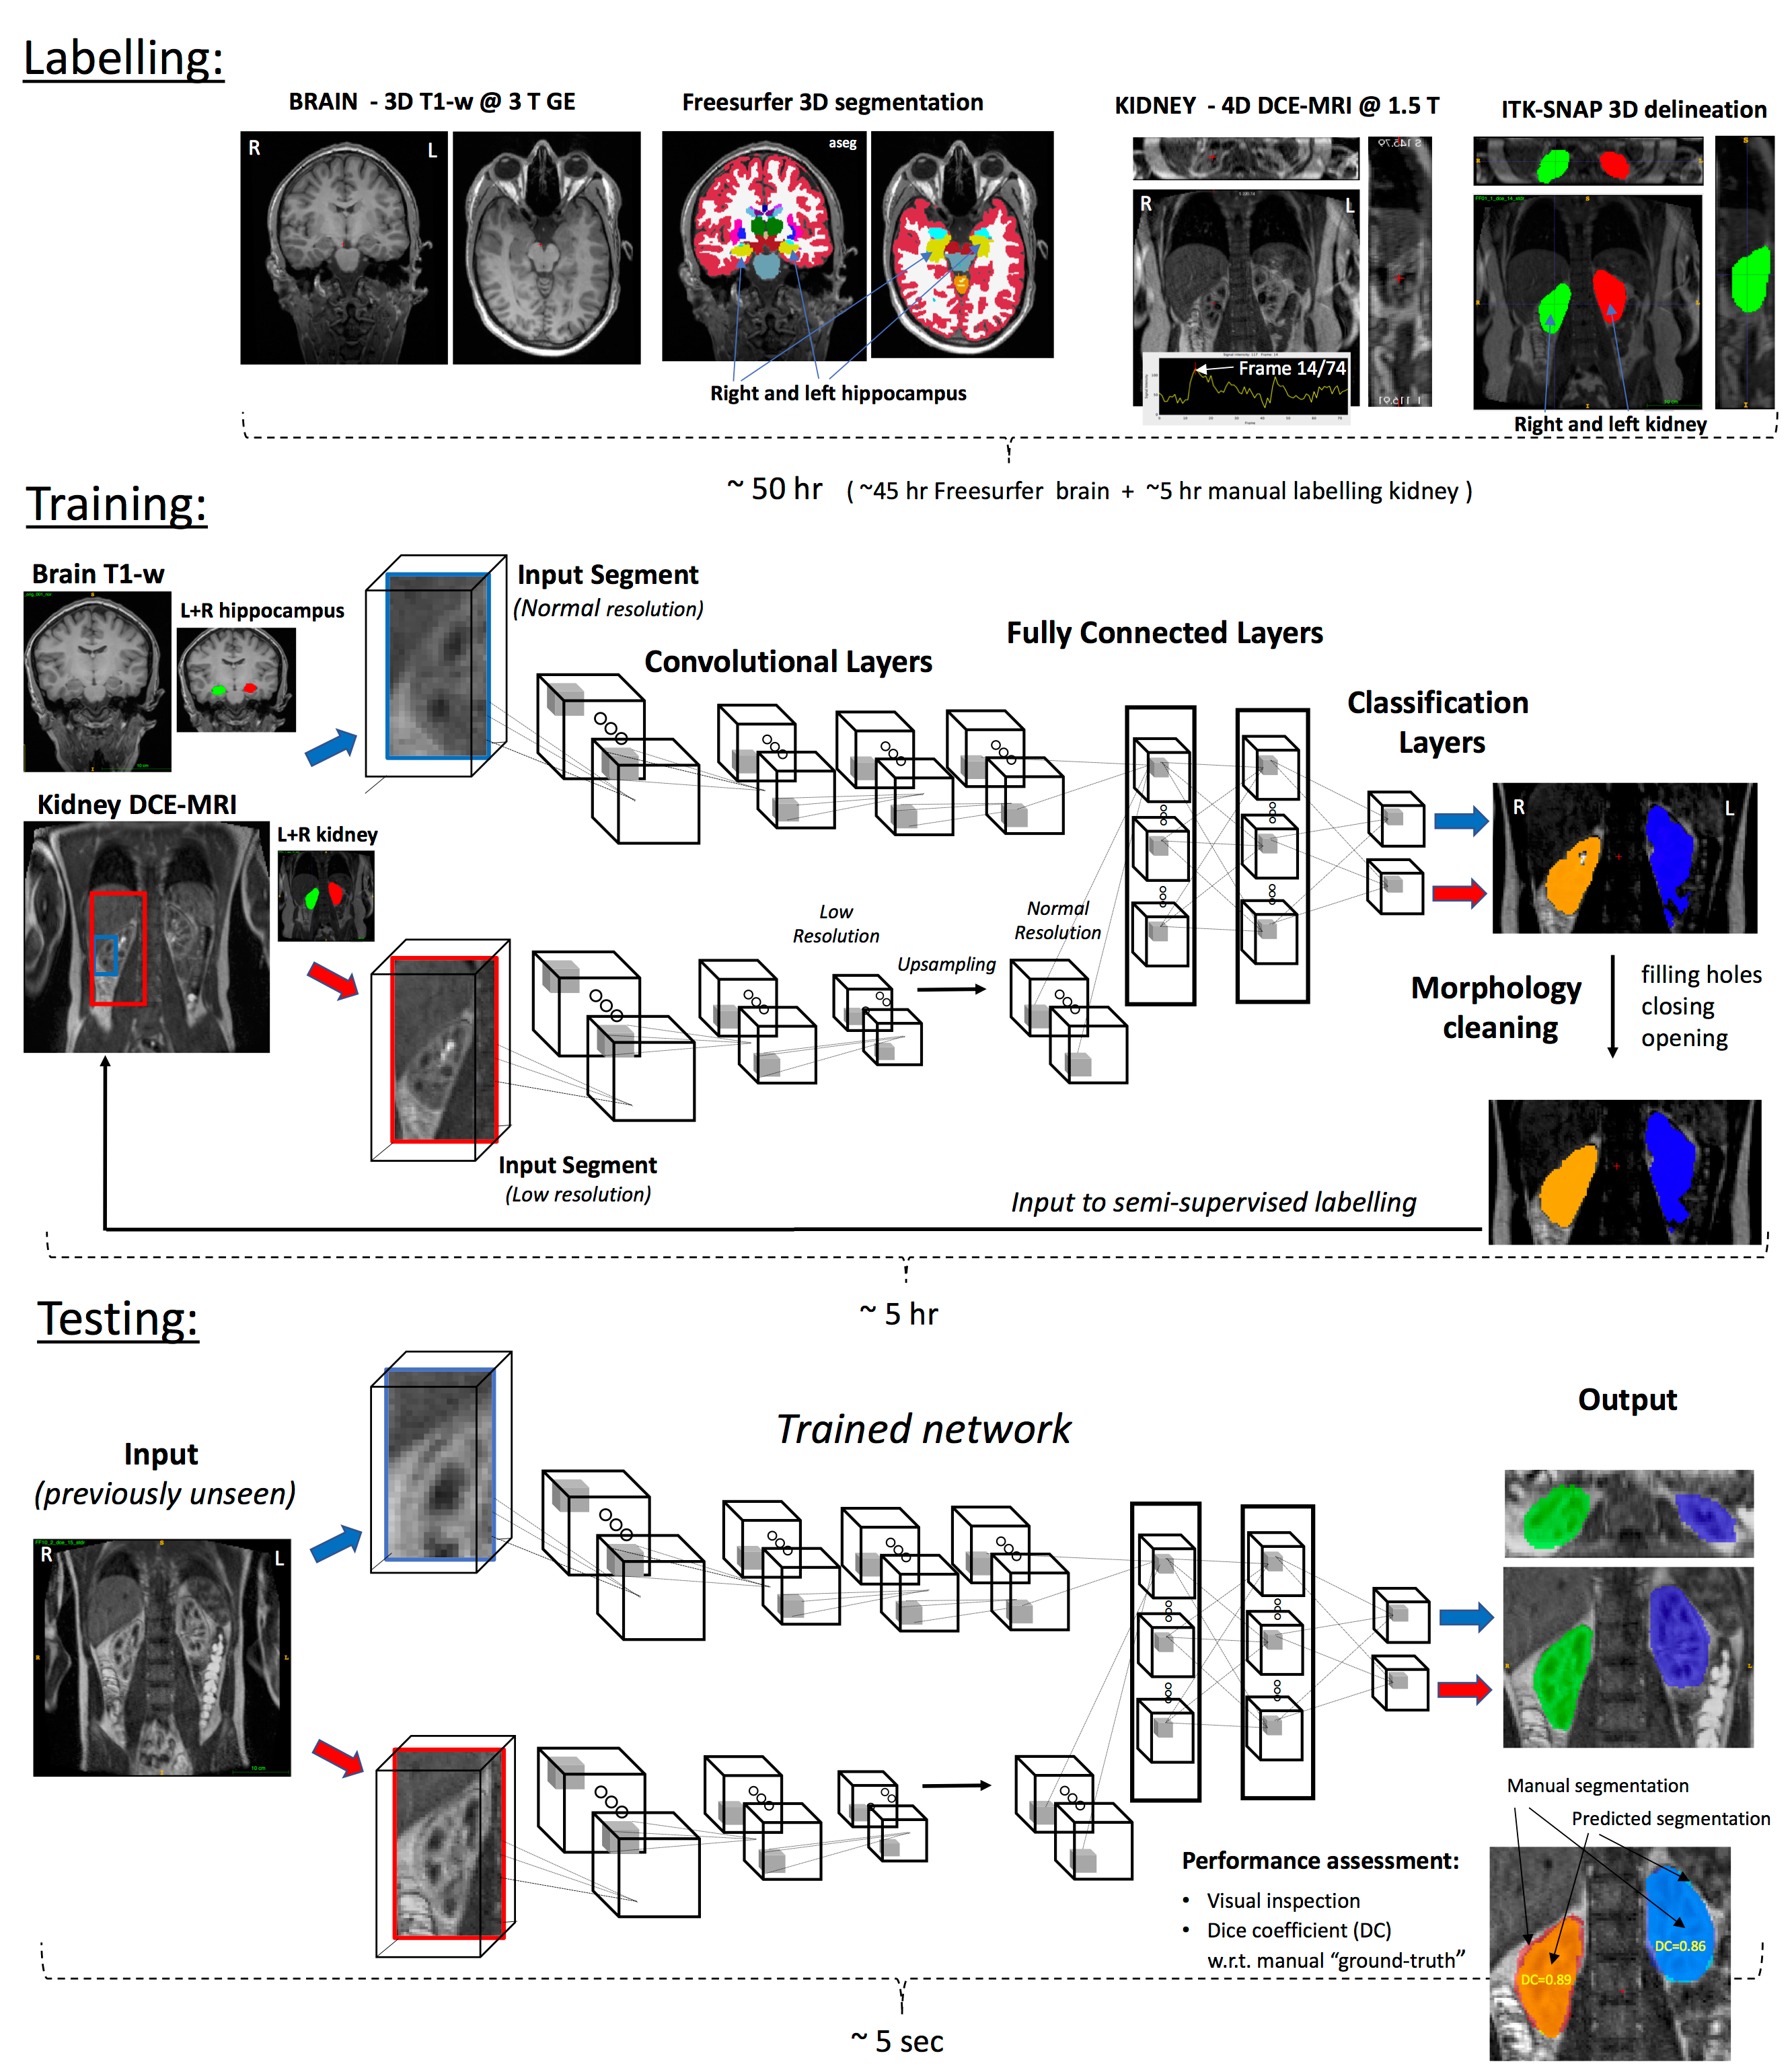
\includegraphics[width = \linewidth]{img/cnn}
	\caption{}
	\label{fig:cnn}
\end{figure*}



\newpage
\subsection{Pharmacokinetic modelling}
The time-dependent distribution and disposition of a substance in a living system can be described by phamacokinetic (PK) models~\cite{gerlowski1983physiologically}. They aim to characterise a physiologic system by decomposing them into interacting compartments. Every of them is a homogenous, well-mixed space with the uniform tracer distribution \cite{PMID:20540902}.




PK models have very wide clinical application: from estimating the optimal drug dose to determining safe working environment while working with toxins  \cite{gerlowski1983physiologically}.
Given the fact that the contrast agent used in DCE-MRI examination can be considered as a substance flowing through the organism, pharmacokintetic modelling can also be used in analysis of so obtained data.   
This approach, called the parametric one, is based on fitting mathematical model to acquired tissue concentration time courses. In this way, the quantitative parameters can be assessed, which cannot be overestimated while evaluating the renal function. 
 

\begin{figure*}[t]
	\centering
	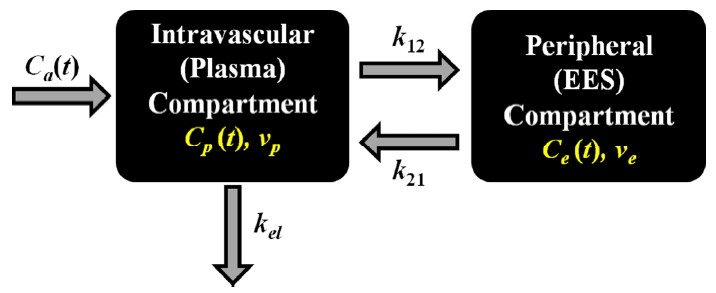
\includegraphics[width = 11cm]{img/diagram2}
	\caption{An example two compartment model \cite{khalifa2014models}.}
	\label{fig:diagram2}
\end{figure*}

The compartment PK models decribe complex blood-tissue exchanges and their theory is based on the differential mass balance equations \cite{sourbron2011tracer}. 
An example of the system decribed by two compartments is presented on Figure \ref{fig:diagram2}.


\subsubsection{Concentration time courses}
  

All PK models used during DCE-MRI analysis require determining both the tissue, $C_t(t)$, and blood plasma, $C_p(t)$, concentration as a~function of time. In our case, the $C_t(t)$ is the mean concentration in renal parenchyma, whereas the
$C_p(t)$, or so called arterial input function (AIF), is a concentration in a blood vessel feeding the kidney (aorta) \cite{khalifa2014models}.  

For each of the kidney, as well as for the aorta, the mean intensities in each time point were calculated. Assuming the linear relation between tracer concentration and signal intensity $S(t)$ \cite{lim2013prediction}, the tracer concentration can be expressed as:


\begin{equation}
	\label{eq:conversion}
	C(t) = S(t)-S(0),
\end{equation}
  
where $S(0)$ is the baseline signal. In order to determine S(0), the time point before rapid signal drop had to be found  as marked on Figure \ref{fig:point}.
%%% Experimenting with two methods, not decided yet %%%%

\textbf{First method:} To do so, for the time course under analysis, the time point in which the derivative of the function reaches the maximal value was selected. 

 
\textbf{Second method:} To do so, for the time course under analysis, time point in which the function reaches the first local minimum $S_{local\_min}$ such that:
\begin{equation}
	\label{eq:local_minimum}
	S_{local\_max} - S_{local\_min} > T_{baseline},
\end{equation}
where $S_{local\_max}$ is the first local maximum occurring after $S_{local\_min}$ and $T_{baseline}$ is threshold empirically set to 15 and 30 for the parenchymal volume and AIF respectively. 
$S(0)$ was then calculated as the mean signal intensity in the initial time interval starting at $T = 0$ to the determined point.

\begin{figure*}
	\centering
	\subfloat[Kidney time course]{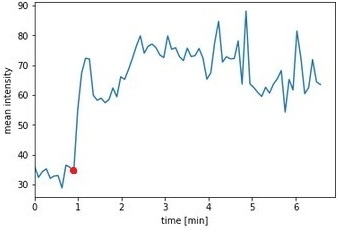
\includegraphics[width=6 cm]{img/timecourse_kidney}}\quad
	\subfloat[Aorta time course]{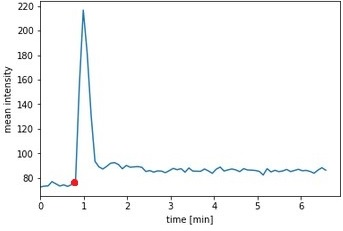
\includegraphics[width=6 cm]{img/timecourse_aorta}}\\		
\caption{Sample average time-courses for renal parenchyma (a) and aorta (b). The last point of baseline is marked with red dot.}
\label{fig:point}
\end{figure*}

Obtained time-concentration curves were then fitted to the described in the next sections PK models.



\subsubsection{Toft's model}
The two compartment Toft's model \cite{tofts1991measurement} assuemes the diffusion of the tracer from the blood plasma at rate specified by the transfer constant $K_{trans}$ $(min^{-1})$ and returns at the rate $k_{ep} = K_{trans}/v_e$ $(min^{-1})$. In this model the assumption $C_t(t) = v_eC_e(t)$ is made, which means that plasma contribution is neglected. The blood plasma concentration $C_p$ is specified by AIF. According to the Toft's model the CA concentraion is specified by the formula:
 
\begin{equation}
	\label{eq:toft}
	C_{t}(t) = K_{trans}\int_{0}^{t}C_p(t')e^{-(K_{trans}/v_e)(t-t')}dt'  
\end{equation}

\subsubsection{Extended Toft's model}
While the Toft's model neglects intravascular contribution assuming weak vascularization of the tissue, the Extended Toft's model \ref{tofts1997modeling} does take it into account. The tissue concentration is described by the formula:
\begin{align}
	\label{eq:extended_toft}
	\nonumber C_{t}(t) &= v_pC_p(t)+\\ 
	&+ K_{trans}\int_{0}^{t}C_p(t')e^{-(K_{trans}/v_e)(t-t')}dt', 
\end{align}
where $v_p$ is the fractional plasma volume. 

In Toft's and extended Toft's models the free parameters $K_{trans}$, $v_e$ and $v_p$ are estimated by fitting the model to obtained in DCE-MRI examinations time concentration curves.  

\subsubsection{Patlak plot}
Another proposed approach is the graphical one called Patlak plot \cite{patlak1983graphical}. Patlak plot neglects $k_{ep}$ due to the low permeability and short examination time. As a result tissue concentration is expressed as:

\begin{equation}
	\label{eq:patlak}
	C_{t}(t) =v_pC_p(t) + K_{trans}\int_{0}^{t}C_p(t')dt'  
\end{equation}
The above equation is the linearised as:
\begin{equation}
	\label{eq:patlak_lin}
	Y = K_{trans}X +v_p,  
\end{equation}
where $Y=C_t(t)/C_p(t)$ and $X=\int_{0}^{t}C_p(t')dt'/C_p(t)$. The free parameters $K_{trans}$ an $v_p$ can be then estimating by constructing a linear plot and calculating its slope and intercept respectively.

\subsubsection{GFR estimation}
Having calculated the $K_{trans}$ parameter the glomelural filtration rate can be computed according to the formula:
\begin{equation}
	\label{eq:gfr}
	GFR = K_{trans}V_{parenchyma}(1-H_{ct}) 
\end{equation}

\begin{figure*}
	\centering
	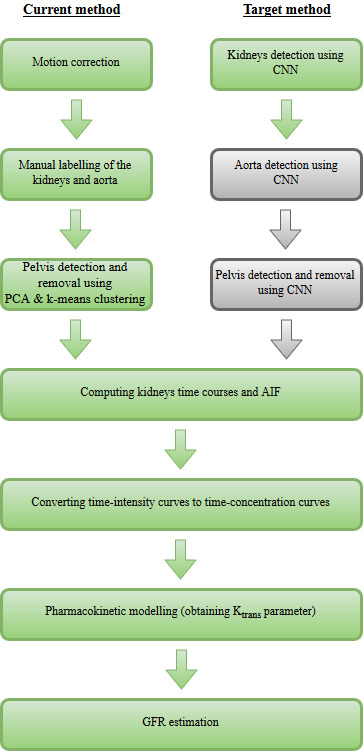
\includegraphics[height = 18cm]{img/methods}
	\caption{}
	\label{fig:methods}
\end{figure*}